%\documentclass[a4paper,9pt,fleqn,notoc]{diss}
%% \renewcommand{\includegraphics}[1][1]{}
%\begin{document}

\chapter{Evolution of Spatial Conceptualization Strategies}\index{alignment}
\label{s:strategies}
In this section I research the question how conceptualization strategies
can form autonomously and align in a population of agents. The previous
chapter studied one component of spatial conceptualization,
namely categorization, in isolation. In this section I take a broader look at  
the prerequisites for building category systems. Every category system
is part of a particular strategy of conceptualizing reality which encompasses
a particular choice of reference objects but also frames of reference and
perspective on the scene. Consequently, which spatial relation system
emerges is governed most importantly by the strategies available to agents.
In the languages of the world different strategies for the 
conceptualization of spatial reality have been attested. This is most strikingly the case 
for frames of reference. Some languages feature only absolute systems, an example being
Tenejapan \citep{levinson2003space}\index{Levinson, S. C.}, while others have developed strong intrinsic and 
relative systems like German \citep{tenbrink2007space}\index{Tenbrink, T.}.
But conceptualization strategies go further. Which objects can function as landmarks?
How are spatial relations applied? What is the role of perspective reversal? 
These are all choices which are manifested in conceptualization strategies and shape
the way a population conceptualizes reality.
Consequently, the evolution of spatial language is intricately linked to the 
emergence and evolution of conceptualization strategies which together
with learning and adaptation operators orchestrate the development of the language system.
To understand the process of building conceptualization strategies this section 
details models of how agents invent strategies and how
they become aligned in the population.

The important claim in this section is that conceptualization strategies 
are negotiated in a cultural process, similar to how the lexicon is negotiated, through local
interactions by agents in a community. The negotiation process is fueled by the 
general cognitive capabilities of agents, in other
words, the cognitive building blocks. Conceptualization strategies package the usage of
certain types of spatial relations with landmarks and perspective. For instance, a conceptualization
strategy might involve a set of spatial relations pertaining to a particular global landmark.
Strategies are represented technically by chunks which are combinations of cognitive operations 
into particular semantic structures that allow agents to conceptualize reality. 
Which strategies are built and which strategies a 
population agrees on in the cultural process is subject to selective pressures that 
influences the preference for a particular strategy over others and drives the 
population to align on a particular way of construing reality. Factors influencing 
invention and alignment\index{alignment} of strategies include primarily environmental conditions such 
as the spatial layout and the kind of objects agents face, but they can also include 
factors such as cognitive complexity of a particular strategy and expressivity
of the language systems developed using that particular strategy. Furthermore,
already established strategies and language systems upon invention
of new strategies influence how and in which way new strategies develop.
The idea is that a particular strategy survives when it is relevant to an agent because
it is efficient and useful in discriminating objects and it contributes to the communicative success of\index{measures!communicative success}
an agent at least in a few spatial contexts. If a new strategy is potentially useful in certain
spatial contexts but in case these spatial situations are already handled by another strategy then
the new strategy has almost no chance of taking over the system unless it performs 
better with respect to other factors such as cognitive complexity. 

In this chapter the focus is on one particular factor governing both invention and alignment \index{alignment}
of strategies: discriminative power. Discriminative power for strategies refers to the distinctive 
ability of a strategy to distinguish and single out objects in the environment. 
Each strategy known to an agent necessarily starts out in a single context.
Which strategy is invented in a particular context is based on its discriminative power
in comparison with other strategies available at that moment. New strategies are packaged into chunks 
and the success of the new strategies is tracked by updating the score of the corresponding 
chunk. So the invention, alignment\index{alignment} and interaction of strategies is structurally organized
very similar to categories. This chapter argues that discriminative power
is an important factor driving the development of strategies, similar to how
it drove the invention and alignment\index{alignment} of spatial categories. In fact, the success
of a strategy is intricately linked to the success of the the category system it builds. 
For instance, if an agent is building a language system with an absolute strategy this 
entails that the absolute relations built using the strategy and the strategy itself
are subject to the same selective pressure. It is the success
of this overall system the spatial relations together with the overall performance
of the strategy that drives the organization of the linguistic and semantic
repository of the agent.

Strategies are implemented using the chunking mechanism of IRL. A particular chunk
represents a particular way of conceptualizing reality. Chunks are invented by
assembling cognitive operations into ready-made semantic structure; they are
scored and their scores are used to represent the success of the conceptualization
strategy over many interactions. Invention operators orchestrate how chunks are
built, and alignment\index{alignment} operators update the score of chunks after interactions tracking
the long-term success of a particular chunk. Spatial conceptualization
strategies rely on spatial relations. Invention of spatial relations is tied to particular 
cognitive operations. For instance, if there is an absolute strategy developed,
the cognitive operation doing the categorization has an associated 
invention operator that invents spatial categories if needed. These are the
same operations as discussed in the last section. Important for the purpose
of this chapter is that this connects the invented spatial relations to
the strategies that incorporate the particular cognitive operation responsible
for invention. 

Before I turn to grammar and other 
linguistic means of expressing strategies, this section focusses entirely 
on alignment\index{alignment} and invention of conceptualization strategies 
without explicit marking in language. In other words, the systems described in
this section are purely expressed through the naming of spatial relations
re-using all of the mechanisms of invention, adoption and alignment\index{alignment} of
spatial categories detailed in the previous section. I apply these
insights on two components of spatial language separately. First,
I study strategies for different reference objects, followed by a discussion of 
the interaction of different frame of reference strategies. Finally the chapter
turns to invention of strategies.

The results presented in this chapter have been published in 
\cite{spranger2011recruitment,spranger2013evolving}.\index{Spranger, M.}

\section{Alignment for Landmark Strategies}\index{alignment}
% reference is unavoidable
Landmarks are an integral part of spatial language
because every spatial relation is implicitly or explicitly related to a reference object.
Typically many different reference objects are present in the world and agents
face choices as to which of the reference objects should be used
in the particular communicative situation but also with respect to invention
and development of language. Environmental conditions can be varied.
In some environments a landmark such as a mountain might be visible in every communicative
encounter between agents of a population which makes it a successful strategy to 
base the spatial language system on this landmark. In other environments
landmarks might only be available locally and its usage, therefore, bound to a particular
communicative encounter. One way of dealing with such choices is that
agents agree on the usage of a particular conceptualization strategy that is 
bound to a particular reference object. This section explores how the use of certain 
reference objects might be aligned in a population of agents. I look at scenes
which feature different landmarks, hence, exhibit a certain amount of choice,
and I study under which circumstances agents are able to align on always using 
the same reference object across spatial scenes. Specifically,
I compare allocentric strategies that are using objects such as boxes
versus egocentric speaker and egocentric hearer strategies. 

The key claim in this section is that conventionalizing a particular strategy of 
conceptualizing reality allows agents to be successful in communication. 
Technically, this claim is studied by setting up systems in which an alignment\index{alignment} strategy is 
implemented that scores semantic structure, more specifically, chunks of semantic structure
and updates the score of semantic structure based on success in communication. 
Chunks that were used in production and interpretation are rewarded
if the interaction was successful and punished if the interaction was a failure. 
Moreover, chunks that were not used in the interaction are punished slightly
which drives the alignment\index{alignment} to find a single strategy most comprehensive strategy that
works in many contexts. This, in essence, implements frequency based dynamics in which structure
that is used successfully survives and structure that is never used or always used unsuccessfully
is removed. Strictly speaking, however, structure is never removed, it just gets a score of zero
which eliminates it from routine processing but leaves it available for recruitment\index{recruitment} should
it become necessary.

The scoring of semantic structure has important consequences. First, the score of a chunk impacts
the choices agents make in production and interpretation. The discrimination score of a chunk, i.e. its discriminatory power given the current context, is multiplied by its score. Consequently,
a speaker might choose to use a less discriminating structure over another because it is 
more conventional, i.e. the score of the chunk is so high as to overrule the discriminative power of the
competitive chunk. Second, the score of a chunk not only governs its usage in a particular spatial context, 
but also influences which categories will be invented. The world from the viewpoint of the
speaker and the hearer might be different from the allocentric viewpoint and, consequently,
the sensori distinctions, i.e. the categories required to be successful using an allocentric strategy 
can be different from those when the same set of scenes is construed from the viewpoint the hearer.
The competition between the conceptualization strategies impacts, in other words, on the particular
category system that will emerge. Because the chunks are under selective pressure, this creates 
a positive feedback loop in which categories might be invented using a particular conceptualization
strategy such as allocentric, which in turn makes this strategy more successful in 
discrimination, which re-enforces the strategy and so on and so forth. 

\begin{figure}
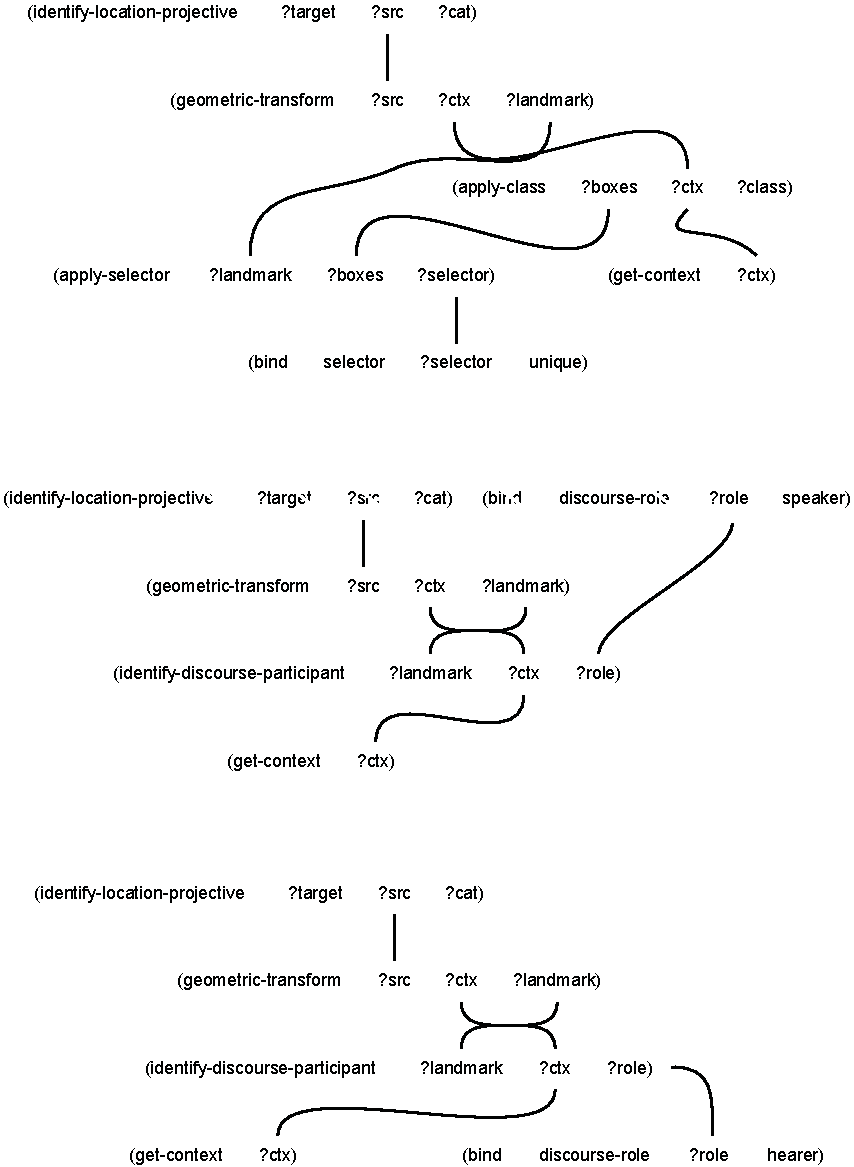
\includegraphics[width=1.0\columnwidth]{figs/chunk-alignment-chunks}
\caption[Conceptualization strategies]{The three conceptualization strategies given to agents. Top: allocentric; middle: egocentric speaker
and bottom: egocentric hearer.}
\label{f:chunk-alignment-chunks}
\end{figure}

\subsection{Experimental Setup and Measures}
I claim that chunk alignment\index{alignment} is an effective mechanism that allows agents to
conventionalize the choice for particular conceptualization strategy alongside 
forming a category system. The claim is tested by running experiments in which agents 
are given different conceptualization strategies: an allocentric strategy 
in which they can use a reference object available in each context, 
and two egocentric strategies one for using themselves and one for using the interlocutor as reference objects
(see Figure \ref{f:chunk-alignment-chunks} for the semantic structures agents are given) . 
At the same time as they are aligning their conceptualization strategy, agents develop a 
category system including names for category distinctions. The category systems and conceptualization
strategies are tightly coupled. Every category is invented as part of a strategy and can only be used
within the strategy it was created in. Success of a particular category in communication,
therefore, directly impacts on the conceptualization strategy. Figures \ref{f:chunk-alignment-acquisition}
and \ref{f:chunk-alignment-formation} show that the mechanism of chunk alignment\index{alignment} works both in acquisition 
and in formation. Agents can successfully negotiate both categories and the 
conceptualization strategy at the same time.

% extra monitoring
The alignment\index{alignment} of conceptualization strategies is measured using the
\emph{conceptualization strategy similarity}\index{measures!conceptualization strategy similarity} which is computed for a population of agents 
by averaging the \emph{agent conceptualization strategy similarity} of every agent to every other
agent. The agent conceptualization strategy similarity $\operatorname{acss}$ is computed by comparing
the score of each strategy. Since strategies are never removed but merely reduced
to a score of $0.0$, one can compute a distance of scores between the chunks in each agent
and envelope the result using an exponential decay function which results in the following formula.
\begin{equation*}
\operatorname{acss}(a_1,a_2,S):=  \exp \left( -1 \cdot \sum_{s \in S} |\operatorname{score}(s,a_1) - \operatorname{score}(s,a_2)| \right) 
\end{equation*}
In this formula $a_1,a_2$ are the agents whose similarity score is computed, $S$ is the set 
of strategies given
to agents and $\operatorname{score}(s,a_1)$ is the score agent $a_1$ gives to strategy $s$.
The conceptualization strategy similarity $\operatorname{css}$ for the population $P$ is defined 
as the average $\operatorname{acss}$
for every two agents. Since $\operatorname{acss}$ is symmetric, all combinations of two agents are
considered. This measure is only one way to understand the dynamics of a particular chunk alignment \index{alignment}
experiment. Since all agents start out equipped with the same set of strategies this measure is equal to $1.0$
in the beginning. However, when considered over many interactions, the measure provides important insights 
into how similar the development is. Particularly, large drops in similarity diagnose significant divergence in strategy use. Most information from $\operatorname{css}$ is drawn by analyzing its dynamics together with a 
second measure which tracks the \emph{average number of chunks} in the population ignoring chunks with a 
score of $0$. If the average number of chunks in a population of agents drops from 3 to 1 and 
$\operatorname{css}$ stays
high, we can conclude that the population has agreed on a single conceptualization strategy (see Figure
\ref{f:chunk-alignment-formation} for such developments). 

\subsection{Results}
Figure \ref{f:chunk-alignment-different-outcomes} shows three different outcomes 
of the chunk alignment\index{alignment} experiments on different data sets. All three graphs show
the average score of the three different strategies over the first 1000 interactions 
of one particular experimental run. All strategies start with 
the same score $0.5$ and for some time nothing happens, because agents 
have not started to invent categories yet. If the first category was invented 
using a particular strategy in a particular context, the strategy that was used 
to invent spreads in the population. Categories invented much later will be 
invented using the dominant strategy, which essentially 
has already been established when the second, third and fourth category 
spread in the population.


\begin{figure}
\begin{centering}
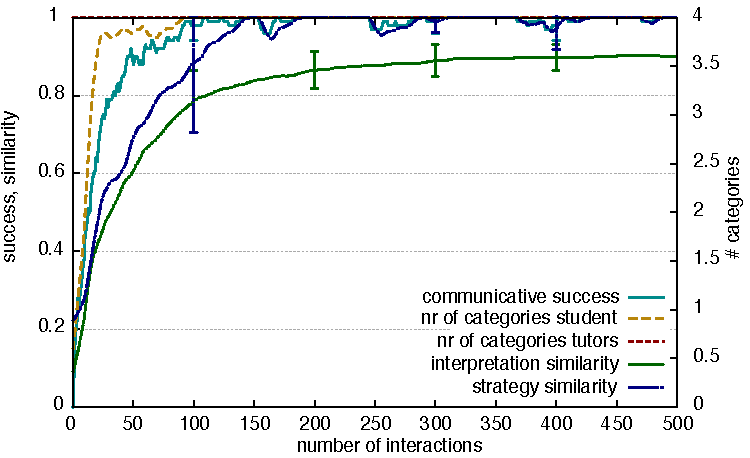
\includegraphics[width=0.9\columnwidth]{figs/chunk-alignment-chunks-acquisition}
\caption[Results strategy acquisition experiments]{
Acquisition experiment in which agents not only learn the 
category system from a tutor (projective in this case), but also 
the underlying conceptualization strategy of the tutor (allocentric).}
\label{f:chunk-alignment-acquisition}
\end{centering}
\end{figure}

\begin{figure}
\begin{centering}
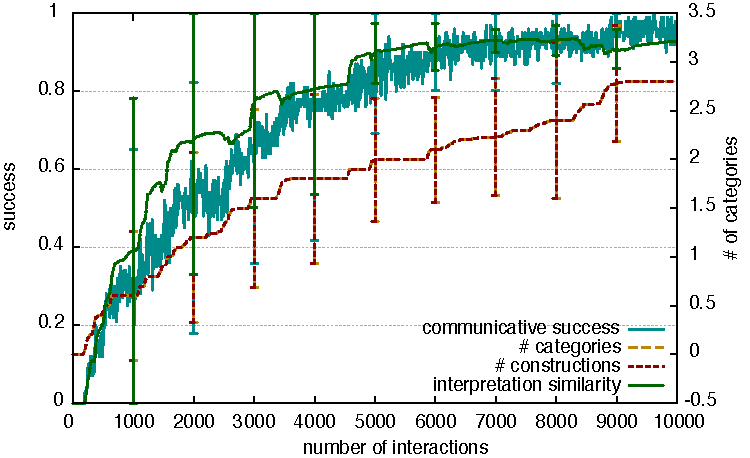
\includegraphics[width=0.85\columnwidth]{figs/chunk-alignment-formation-projective-space-game-5-success}
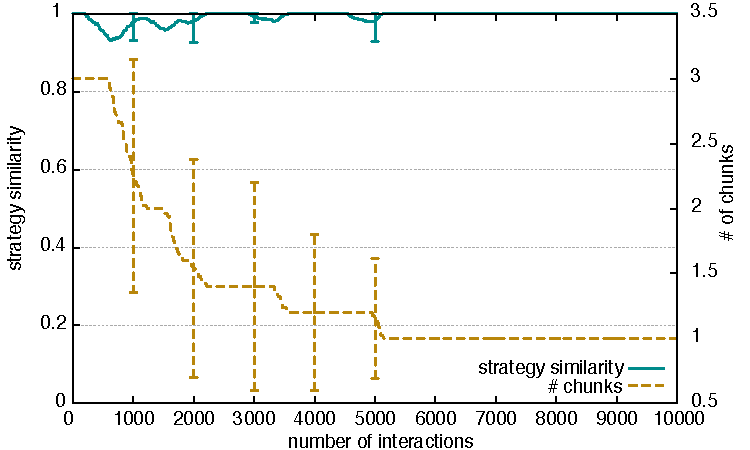
\includegraphics[width=0.85\columnwidth]{figs/chunk-alignment-formation-projective-space-game-5-alignment}
\caption[Results for conceptual alignment]{Experimental results for conceptual alignment\index{alignment}. In these experiments 10 agents
are negotiating conceptualization strategies while at the same time agreeing on a system of 
spatial relations. The top shows the development of categories and communicative success\index{measures!communicative success}. 
The dynamics is quite similar to previous experiments using a dampened invention 
approach to categorization. The bottom figure shows that for this particular data set one 
specific strategy always unanimously wins the competition. which can be seen both by the 
drop to a single chunk and the corresponding high strategy similarity. Strategy 
similarity starts out high because all agents start 
with the three strategies, but most importantly, it also stays high suggesting high similarity between
the conceptualization strategies agents are using.
}
\label{f:chunk-alignment-formation}
\end{centering}
\end{figure}

\begin{figure}
\begin{centering}
%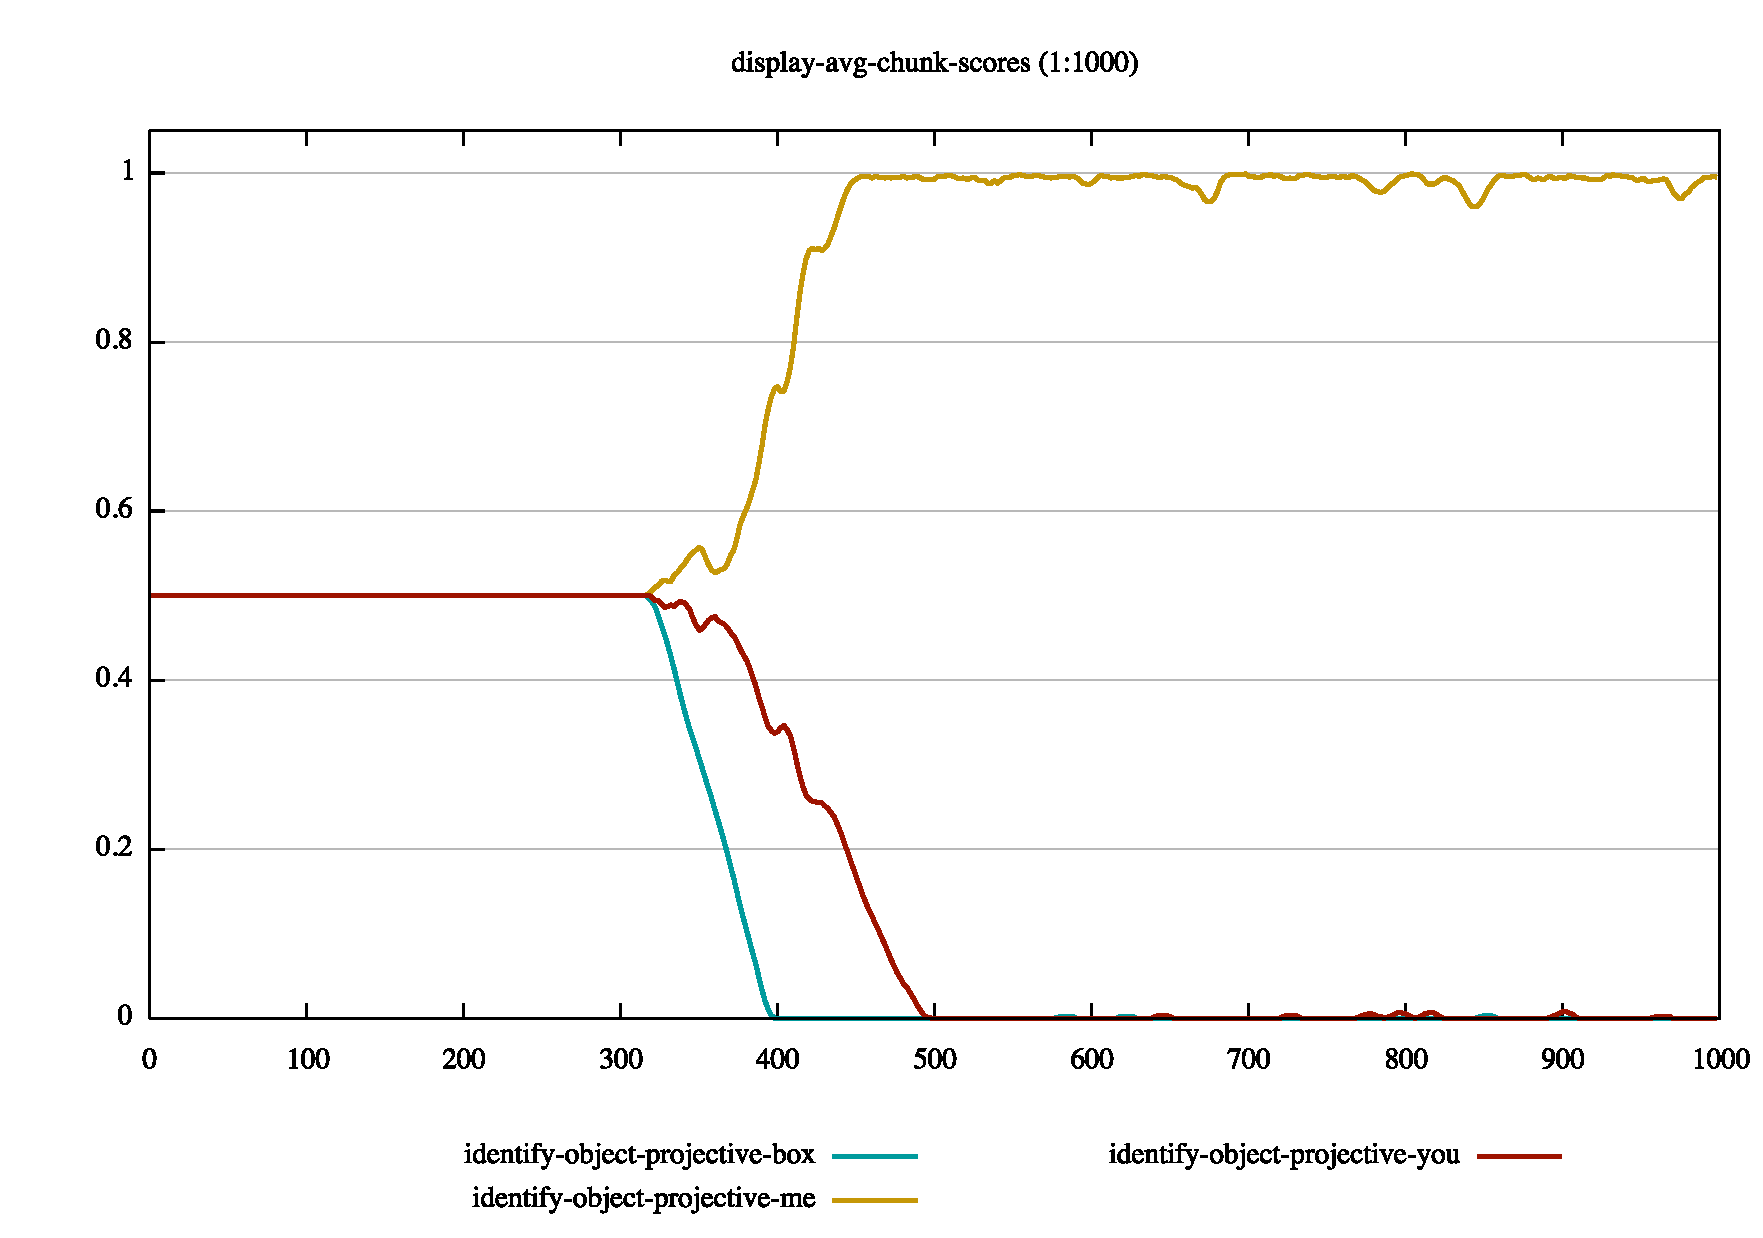
\includegraphics[width=0.65\columnwidth]{figs/chunk-alignment-formation-projective-space-game-4-run-1}
%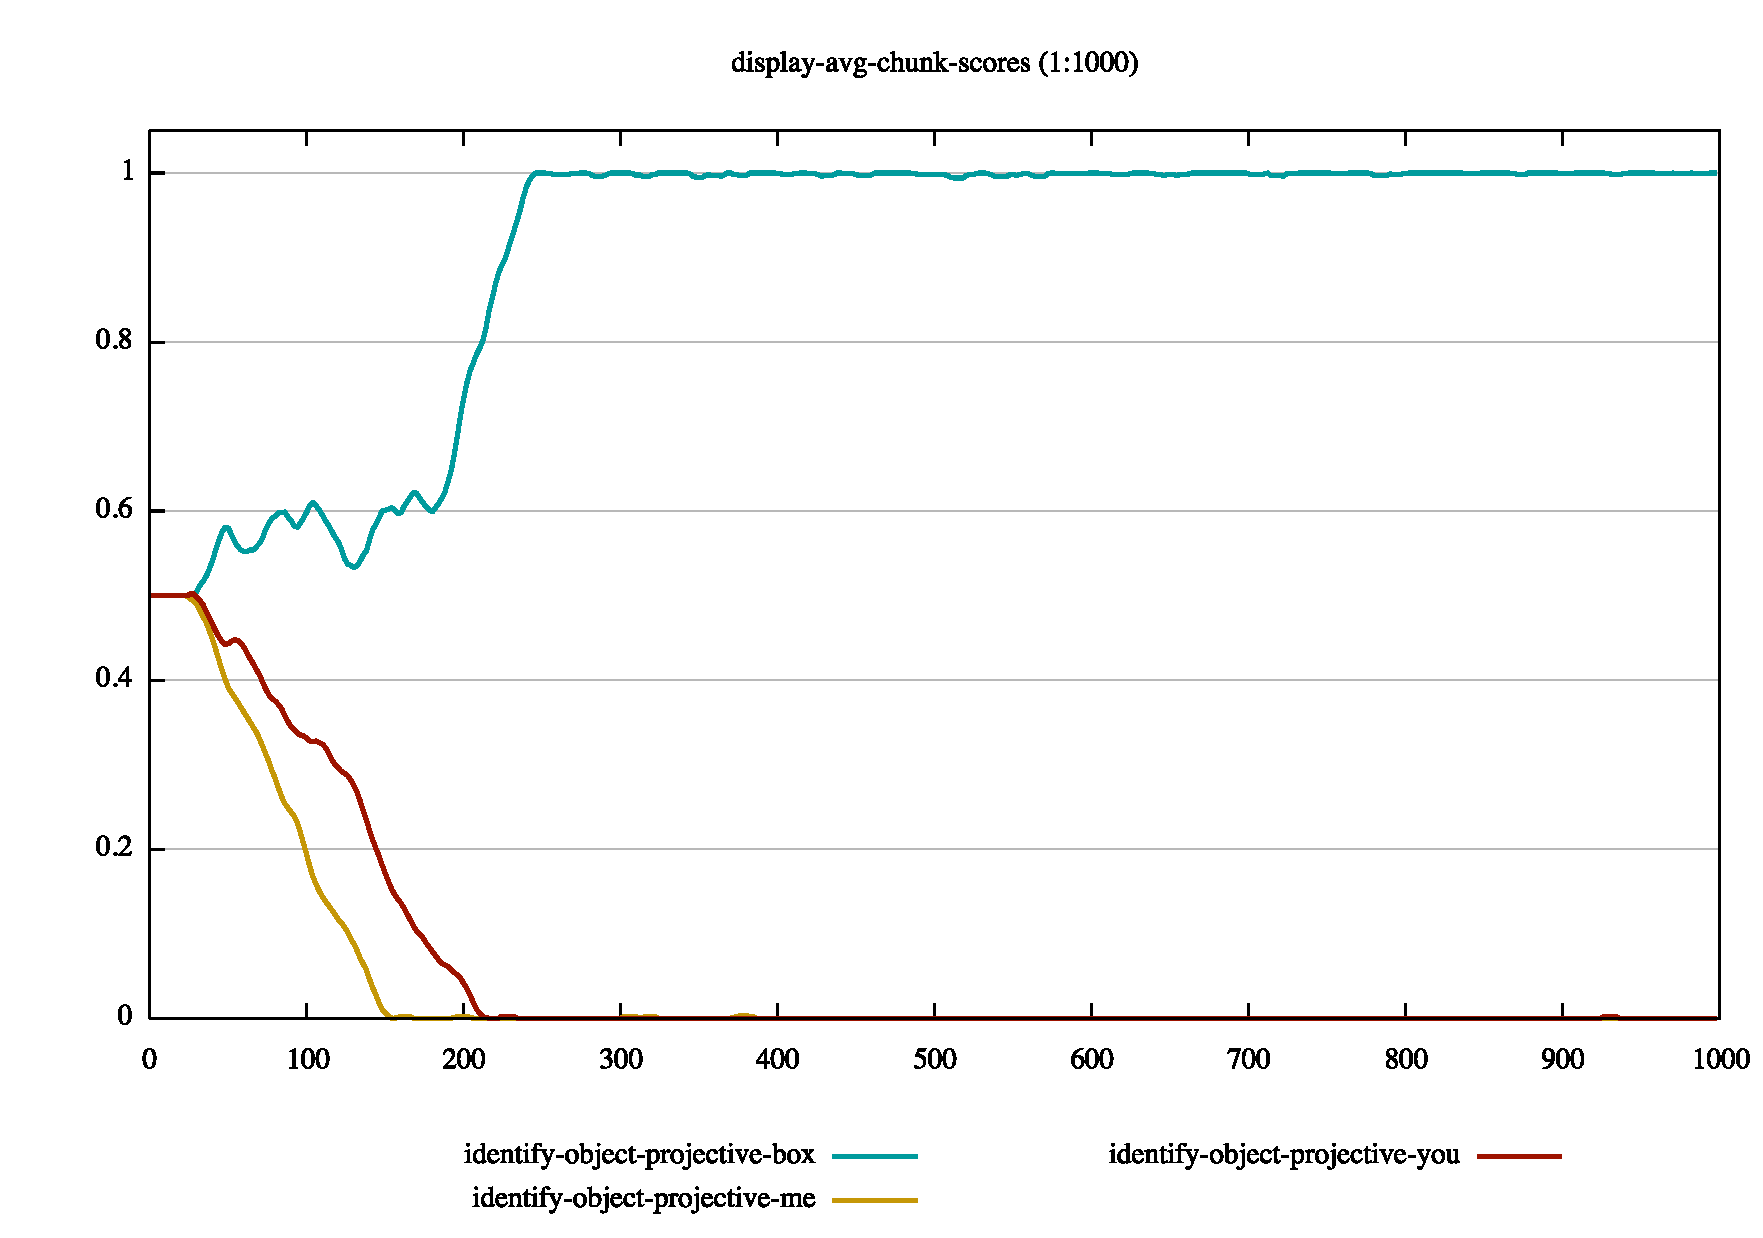
\includegraphics[width=0.65\columnwidth]{figs/chunk-alignment-formation-projective-space-game-4-run-2}
%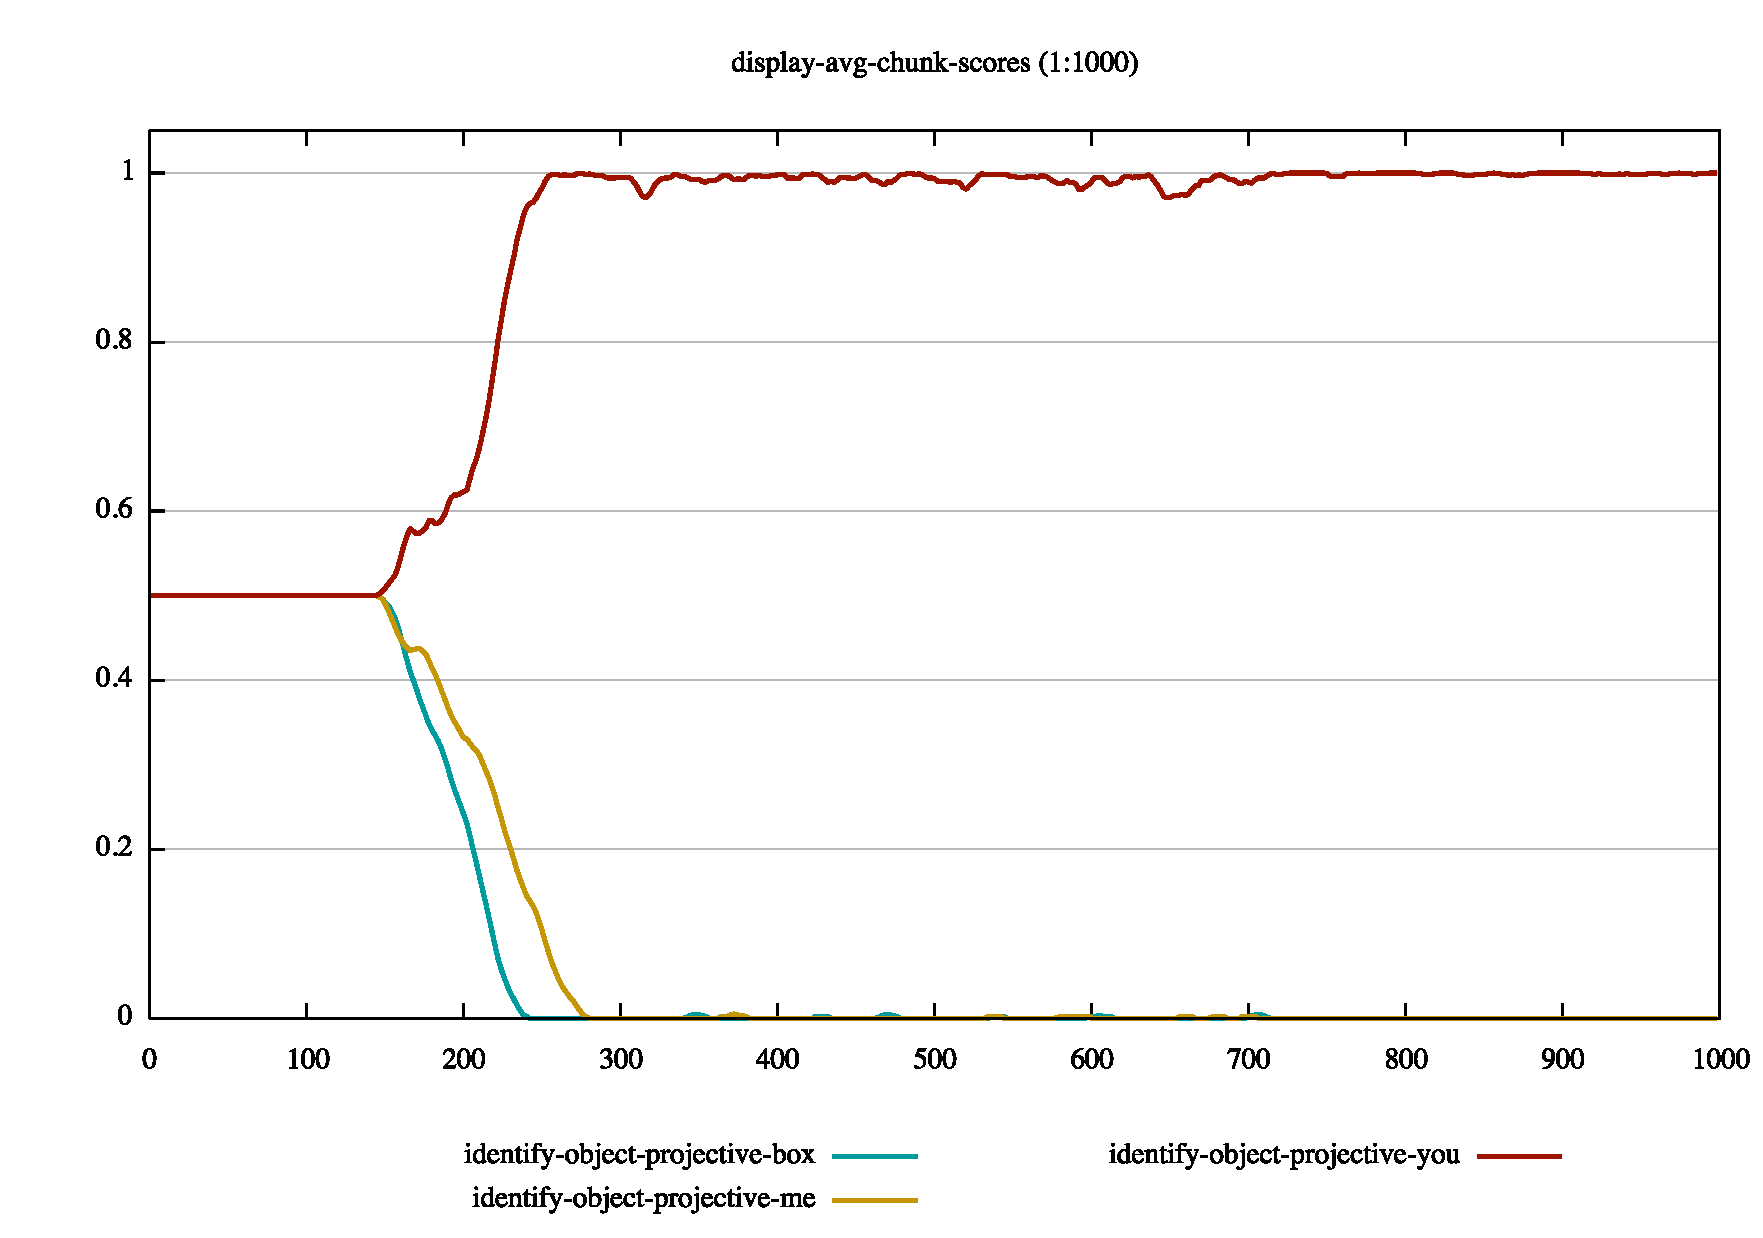
\includegraphics[width=0.65\columnwidth]{figs/chunk-alignment-formation-projective-space-game-4-run-3}
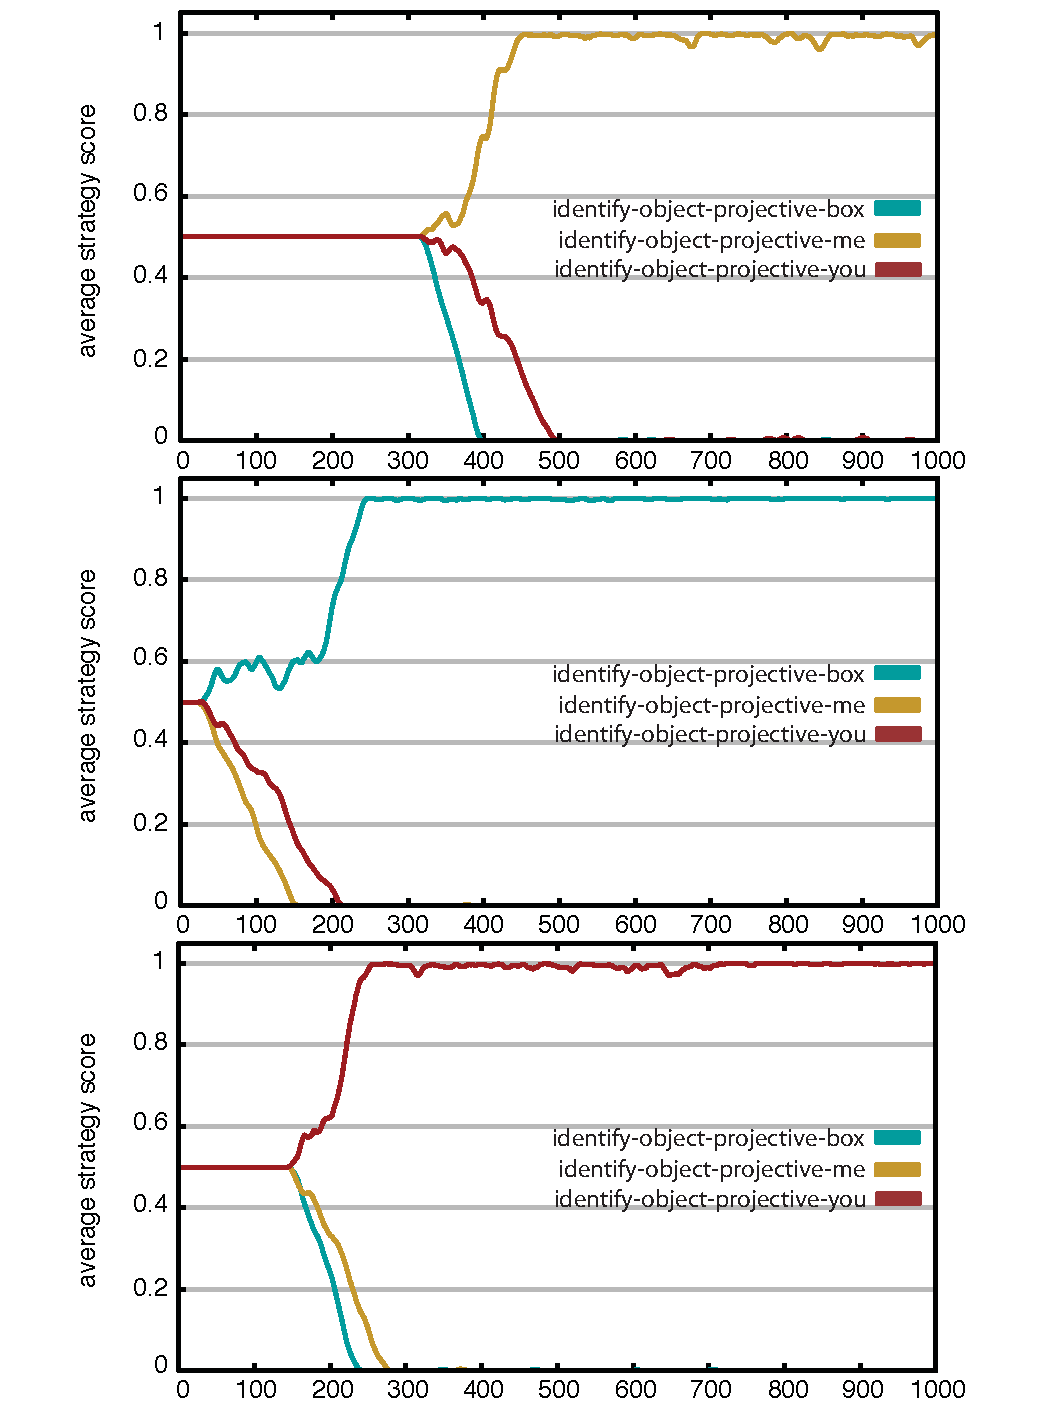
\includegraphics[width=0.95\columnwidth]{figs/chunk-alignment-formation-projective-space-game-4-together}
\caption[Different outcomes of chunk alignment experiments]{
Different outcomes of the chunk alignment\index{alignment} experiments on 
different data sets. All three graphs show the average score of the three different 
strategies over the first 1000 interactions of one particular experimental run. 
Top: the speaker egocentric strategy survives; middle: allocentric strategy 
wins and right: the hearer egocentric strategy wins.}
\label{f:chunk-alignment-different-outcomes}
\end{centering}
\end{figure}


The choices in alignment\index{alignment} of strategies depend on the discriminative advantage of the strategy. 
This is a subtle effect which can easily lead to unaligned populations particularly because
agents simultaneously develop categories which is a powerful and adaptive mechanism.
The problem lies in adoption. If the hearer observes a new term,
the only information given to him in order to decide which strategy to use for adoption is the current
context and its particular spatial layout. Let us suppose the speaker thinks the conventional 
strategy in the population is allocentric and, consequently he uses an allocentric spatial
category. If the context is indeed one that favors the allocentric strategy, there is no problem and
the hearer will correctly adopt the category as allocentric. If, however, the context favors a
conceptualization strategy from the viewpoint of the hearer and the hearer does not share the 
strong preference for the allocentric strategy with the speaker, he will adopt the term as 
part of a hearer strategy. Even though the category is essentially unaligned
because different agents see it as part of different strategies, it might still be quite successful, 
particularly in context where there are few objects. 
If success of the category is above $50\%$, it is very hard for the alignment\index{alignment} mechanisms 
to remove it, since success is rewarded much more than failure is punished to allow 
the system to get off the ground. In such cases, misalignment can appear while retaining
success rates of above $50\%$ in communication. In other words, agents might get stuck in 
local optima and without additional mechanisms might be unable to get out of such
conditions.

%Lastly, we can consider one particular parameter of the system which is the close coupling
%of categories and conceptualization strategies. So the question is what if that coupling
%is less strict. What is clear is that typically language systems are developed for a very specific
%purpose and then potentially over time they grow to fulfill different functions widening their 
%area of application. For spatial language paths from body parts to egocentric to allocentric
%developments have been sketched and attested in the literature... So does not seem implausible
%to assume a strong coupling between the strategy and the categorization system it invents.
%But how these two components of conceptualization precisely interact is far from being
%determined conclusively which leaves the question of modeling...

%
%In the most extreme case of no coupling, categories invented in one strategy will
%be immediately available for use in other strategies just because they rely
%on the same cognitive operations.


\section{Alignment for Frame of Reference Strategies}\index{alignment}
The same mechanisms explaining alignment of reference object conceptualization strategies 
can be used to explain the alignment of
other components of spatial language such as frames of reference, e.g. intrinsic and absolute
conceptualization strategies. The claim is that agents can deal 
with the problem of aligning frames of reference by aligning chunks based on environmental 
conditions that favor one over the other. Particularly, I revisit the problem discussed
in Sections \ref{s:category-acquisition} and \ref{s:category-formation} which argued
that agents who are equipped at the same time with projective and absolute 
strategies are unable to develop category systems without clear preferences for one of the 
two strategies. Here, I turn to the question how such preferences can develop from
scratch based on the long-term tracking of the success of each strategy. 
Just as for reference objects, I study environmental conditions 
and their impact on the success of strategies. 


% absolute and intrinsic revisited
To understand the impact of environmental conditions, we have to understand the pre-requisites
for the two strategies at hand. The absolute strategy requires the environment
to exhibit absolute features such as a global landmark. The global landmark must be present
in some contexts and it must help to discriminate objects in the context. That is to say,
in environmental conditions where there are no absolute landmarks or the direction
to the absolute landmark is not discriminating, agents do not develop an absolute system.
For intrinsic systems the environment, most specifically the landmark objects that are used
in conceptualization, have to have properties that allow to conceptualize a direction with respect
to the reference object. So one can conclude that in environments were landmarks do not have an 
orientation or where the direction of objects in each context is not discriminating with respect to the
orientation of landmark objects, no intrinsic system will develop. A word of caution is at place here,
I will talk about the environment as having intrinsic or absolute features. This is in many ways
loose talk, as it is never the environment that has such features but rather the environment is 
conceptualized by humans or robots as having such features and it is never the environment itself
that has an absolute landmark or a landmark with intrinsic features. Now, a mountain range or any
other feature of some environment may license or in some ways encourage agents to use the object
as a global feature, but, certainly, the decision as to what counts as a global feature is still part of an active
cognitive process. This process is simulated, here, by manipulating the spatial context to include
an absolute landmark or a landmark that has an inherent orientation. Hence, I talk loosely
about environmental conditions pertaining to absolute and intrinsic features, but readers have
to keep in mind that this really is scaffolding much more complex processes.

% interaction of strategies
The strategies an agent possesses always interact in local communicative interactions.
Usage of a particular strategy in production, interpretation and invention of spatial relations
is exclusively governed by the discriminative power of each strategy. 
In cases where the discriminative power of two strategies is equal, this leads to a problem in the
sense that the agent cannot decide which strategy to use. 
This problem is especially pressing when agents have not started inventing spatial relations yet and need to decide which
strategy to use. This sort of situation 
is precisely the problem occurring when intrinsic 
and absolute systems interact in conditions that license both. In order for agents to successfully 
develop a category system, the symmetry of equal discriminative power of intrinsic and absolute 
categories, must be broken. The mechanisms for alignment\index{alignment} of conceptualization strategies can
help break this symmetry by tracking the success of each strategy. Even if only in a few contexts
there is a clear advantage for one of the strategies, the scoring of conceptualization strategies 
allows agents to track this advantage at which point the success can carry over to 
contexts that license no particular preference. For instance, if one context out of many
features only an absolute landmark and no intrinsic features, agents use this context
to start an absolute category system at the same time rewarding the absolute conceptualization
strategy. This initial reward carries over to other contexts which feature both intrinsic and
absolute features. The head start of the absolute strategy then leads to additional 
absolute spatial relations being developed which in turn make the absolute system
more successful in communication rewarding both the individual absolute relations as
well as the overall strategy. In this way the local discriminative power 
leads to consensus on the population level over time as to which strategy to use. 
The alignment\index{alignment} on the population level can override the particular discriminative power 
of strategies in some specific context. That is to say, once there is an established strategy 
within the population, it gets chosen even in cases where
another strategy would be more discriminating or equally discriminating.

\begin{figure}
\begin{center}
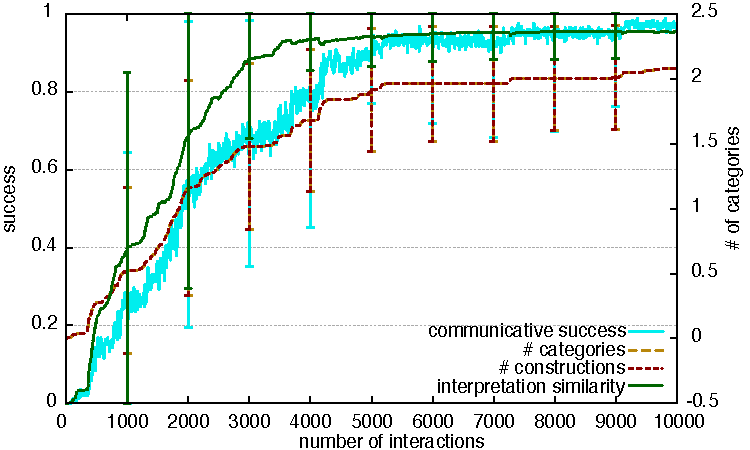
\includegraphics[width=0.9\columnwidth]{figs/chunk-alignment-frames-absolute-vs-intrinsic}
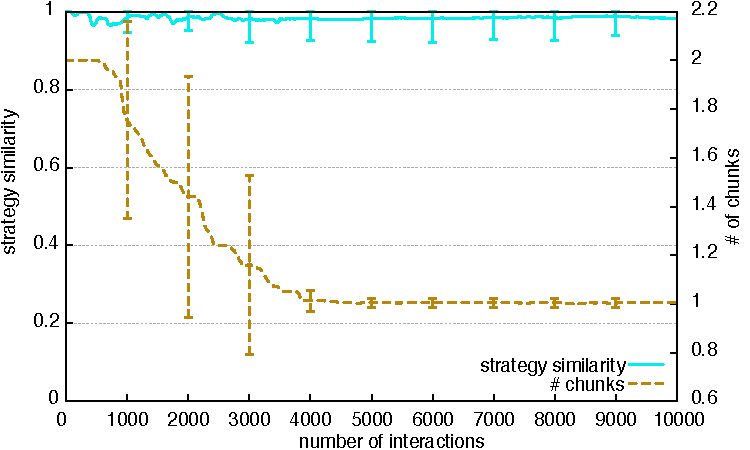
\includegraphics[width=0.9\columnwidth]{figs/chunk-alignment-frames-absolute-vs-intrinsic-alignment}
\end{center}
\caption[Results category formation and frame of reference alignment\index{alignment}]{
Dynamics of a category formation experiment in which 10 agents align the frame of reference
used in conceptualization. The environment has a clear preference for the absolute frame of reference
in that it is the only frame of reference available in certain context. 
In $50\%$ of the contexts both intrinsic and absolute
frame of reference are available, in the remaining $50\%$ of the contexts only an absolute frame
of reference is available. The strong preference of the environment drives agents to develop 
an absolute system which dominates across 25 runs of the same experiment. The graph shows 
that together with the category system agents align their conceptualization strategy.}
\label{f:chunk-alignment-frames-absolute-vs-intrinsic}
\end{figure}



\subsection{Experimental Setup}
I test the power of chunk alignment\index{alignment} using contexts which can be manipulated to feature 
absolute and intrinsic properties. More specifically, I manipulate the distribution of intrinsic and 
absolute properties in the environment. Figure \ref{f:chunk-alignment-frames-absolute-vs-intrinsic} 
shows the dynamics of an experiment where agents start equipped with two strategies: an absolute
and an intrinsic one. The environment is such that it favors absolute systems. In $50\%$ of the 
scenes both intrinsic and absolute features are present. In the remaining $50\%$ of the contexts
only absolute features are present and no intrinsic ones. The environmental
conditions have a strong effect on the development of the system in that all 25 populations
agree on using an absolute strategy. What is important is that the contexts where
only absolute features are present reward the absolute strategy and punish the intrinsic 
conceptualization strategy. Consequently, even in contexts where intrinsic and absolute features 
are present, the absolute strategy is preferred. The development of such a preference
has important effects on the invention of categories. Because of the preference for 
the absolute strategy, invention of categories shifts to producing only absolute categories.
The successful use of these categories enforces the absolute strategy and leads to further
punishment of the intrinsic strategy. The effect is that only the absolute strategy survives.

\subsection{Results}
The influence of the distribution of features in the environment and its impact
on the developing system are shown in Figures 
\ref{f:chunk-alignment-frames-absolute-vs-intrinsic-bar-plot} 
and \ref{f:chunk-alignment-frames-absolute-vs-intrinsic-detail}. 
Both figures show results for different experimental conditions. In all conditions
$50\%$ of the scenes feature both intrinsic and absolute properties. The conditions
differ only in how the remaining $50\%$ of  scenes are divided. The following table
overviews the conditions.
\begin{center}
    \begin{tabular}{ | l | p{1.5cm} | p{1.5cm} | p{1.5cm} |}
    \hline
    condition & both & intrinsic only & absolute only \\ \hline\hline
    0.0 & 50\% & 0\% & 50\%\\ \hline
    0.25 & 50\% & 12.5\% & 37.5\% \\ \hline
    0.50 & 50\% & 25\% & 25\% \\ \hline
    0.75 & 50\% & 37.5\% & 12.5\% \\ \hline
    1.0 & 50\% & 50\% & 0\%\\ \hline
    \end{tabular}
    \label{t:conditions}
\end{center}
Conditions are named after the percentage of intrinsic only scenes in the $50\%$ of scenes that
feature either only intrinsic or only absolute properties. 
Figure \ref{f:chunk-alignment-frames-absolute-vs-intrinsic-detail} shows the average 
score of the absolute and intrinsic strategies (projective).  
In all three cases, $50\%$ of the scenes feature both intrinsic and absolute properties. 
On the top results are shown for an environment that in the remaining $50\%$ has only 
absolute features. The middle figure shows results where 
$25\%$ have only absolute features and $25\%$ only intrinsic features. 
The bottom figure shows results for $50\%$ intrinsic features. Clearly, agents in all 
cases align strategies reflecting environmental conditions. If the environment clearly 
supports an absolute strategy, the absolute strategy wins. If there are clear advantages 
for having an intrinsic strategy (bottom), the intrinsic strategy takes over and suppresses 
the absolute strategy.


Figure \ref{f:chunk-alignment-frames-absolute-vs-intrinsic-bar-plot} compares communicative success
as well as resulting average scores of each strategy. Interestingly, the middle condition $0.5$ exhibits
a significant drop in communicative success to around $80\%$. The reason for this can be seen in Figure 
\ref{f:chunk-alignment-frames-absolute-vs-intrinsic-detail} (middle) which shows the dynamics
of a single run of such an experiment. In this condition no strategy is particularly favored and to
be reasonably successful both strategies are necessary. This leads to both strategies having
high scores. In a particular moment of inventing a new category both agents might have slightly
different preferences for strategies based on their respective recent history of interaction.
One agent might have just used the intrinsic strategy successful, whereas the other has
just the absolute strategy. In this situation, invention happens wrongly in the sense that one
agent might invent an absolute category and the other adopt it as an intrinsic strategy.
Such categories which have different types across the population are the cause of the drop
in success. Overall, however, the system is able to self-organize under different conditions and successful
communication systems emerge.

\begin{figure}
\begin{center}
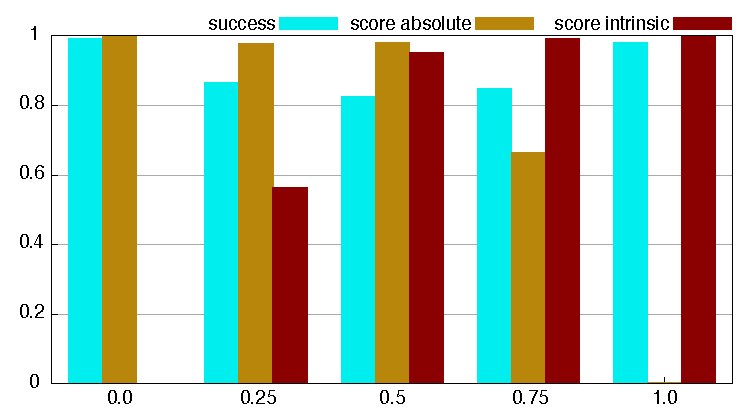
\includegraphics[width=1.0\columnwidth]{figs/chunk-alignment-frames-absolute-vs-intrinsic-bar-plot}
\end{center}
\caption[Comparison for different distributions of intrinsic and absolute features]{
Results for experiments with different distributions of intrinsic and absolute features. Each condition
was tested with 25 experiments of populations with 10 agents each. The figure shows the 
communicative success\index{measures!communicative success} and the scores of the absolute and intrinsic strategy averaged over the
multiple runs.}
\label{f:chunk-alignment-frames-absolute-vs-intrinsic-bar-plot}
\end{figure}


\begin{figure}
\begin{center}
%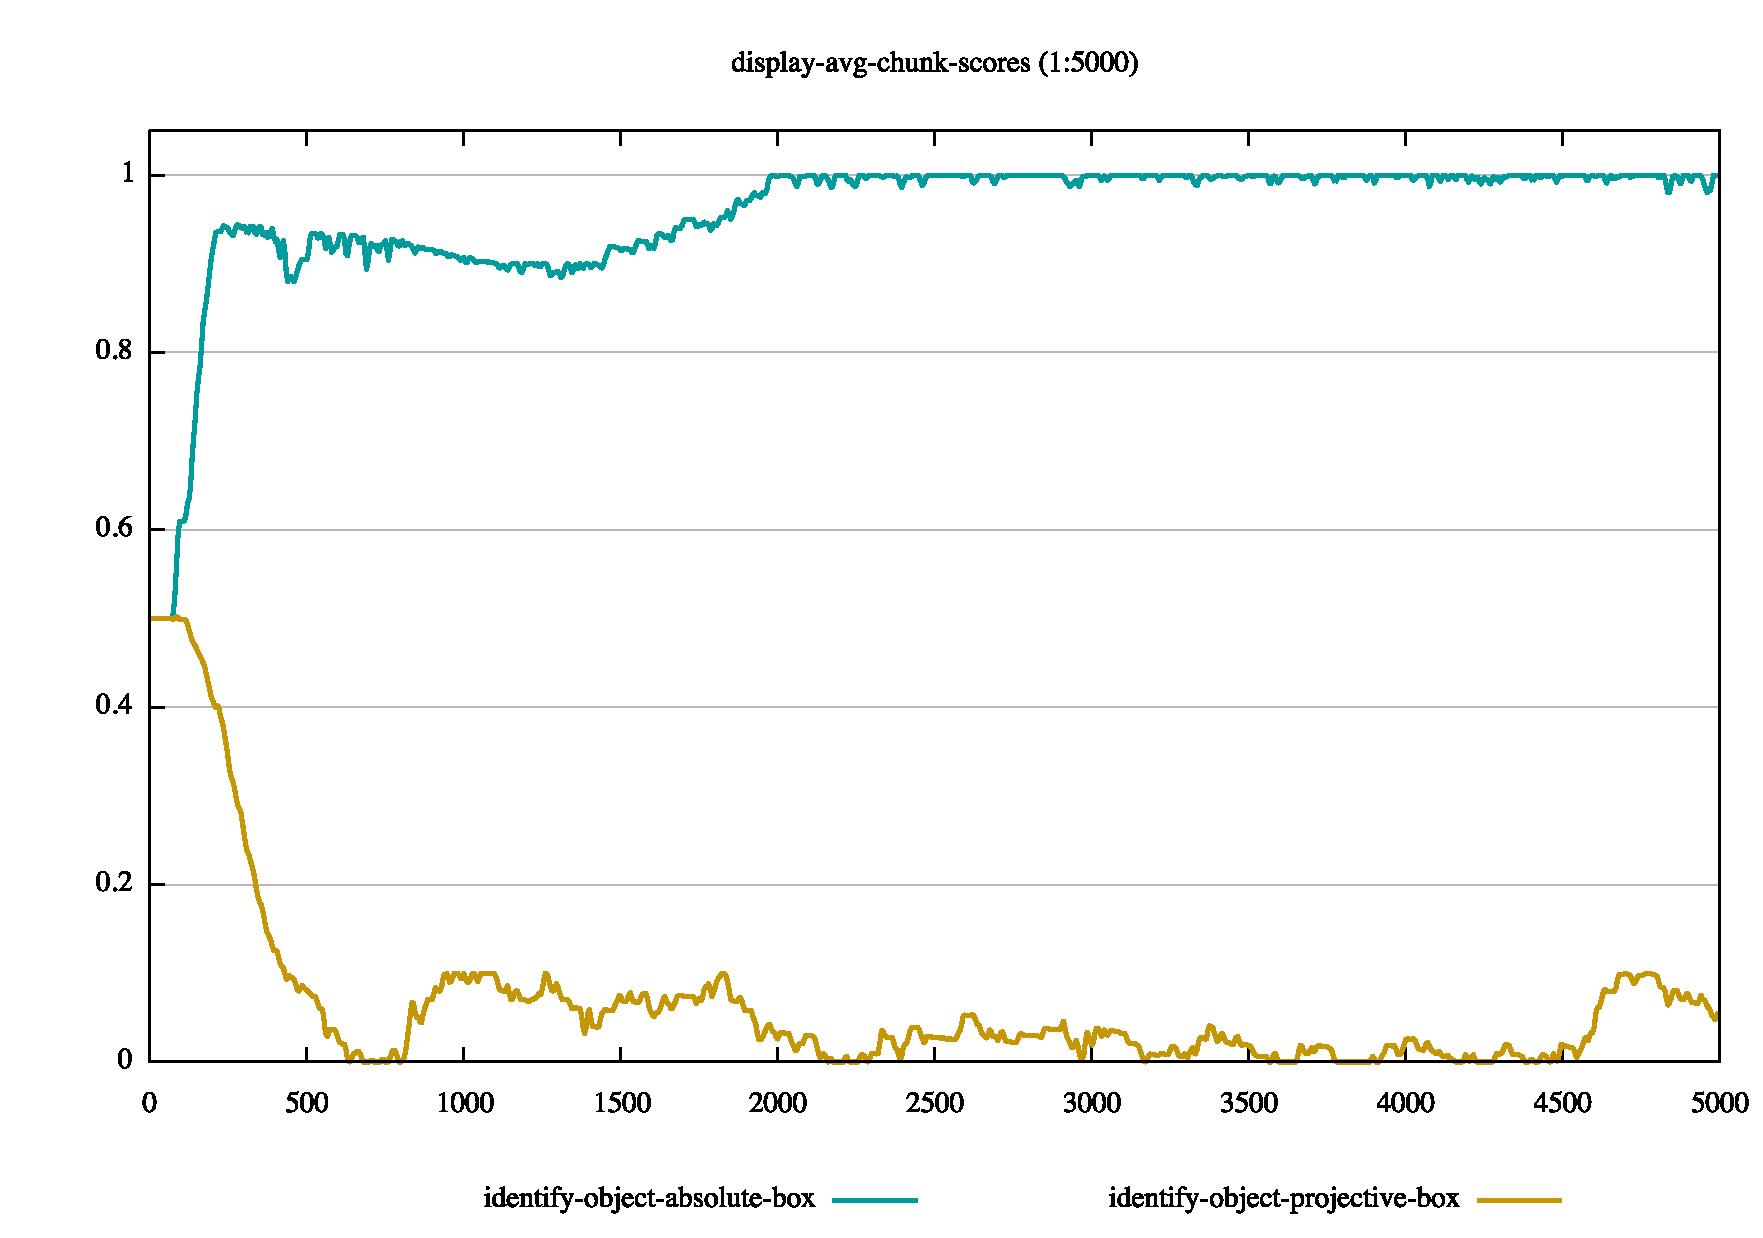
\includegraphics[width=0.7\columnwidth]{figs/chunk-alignment-frames-absolute-vs-intrinsic-00.pdf}
%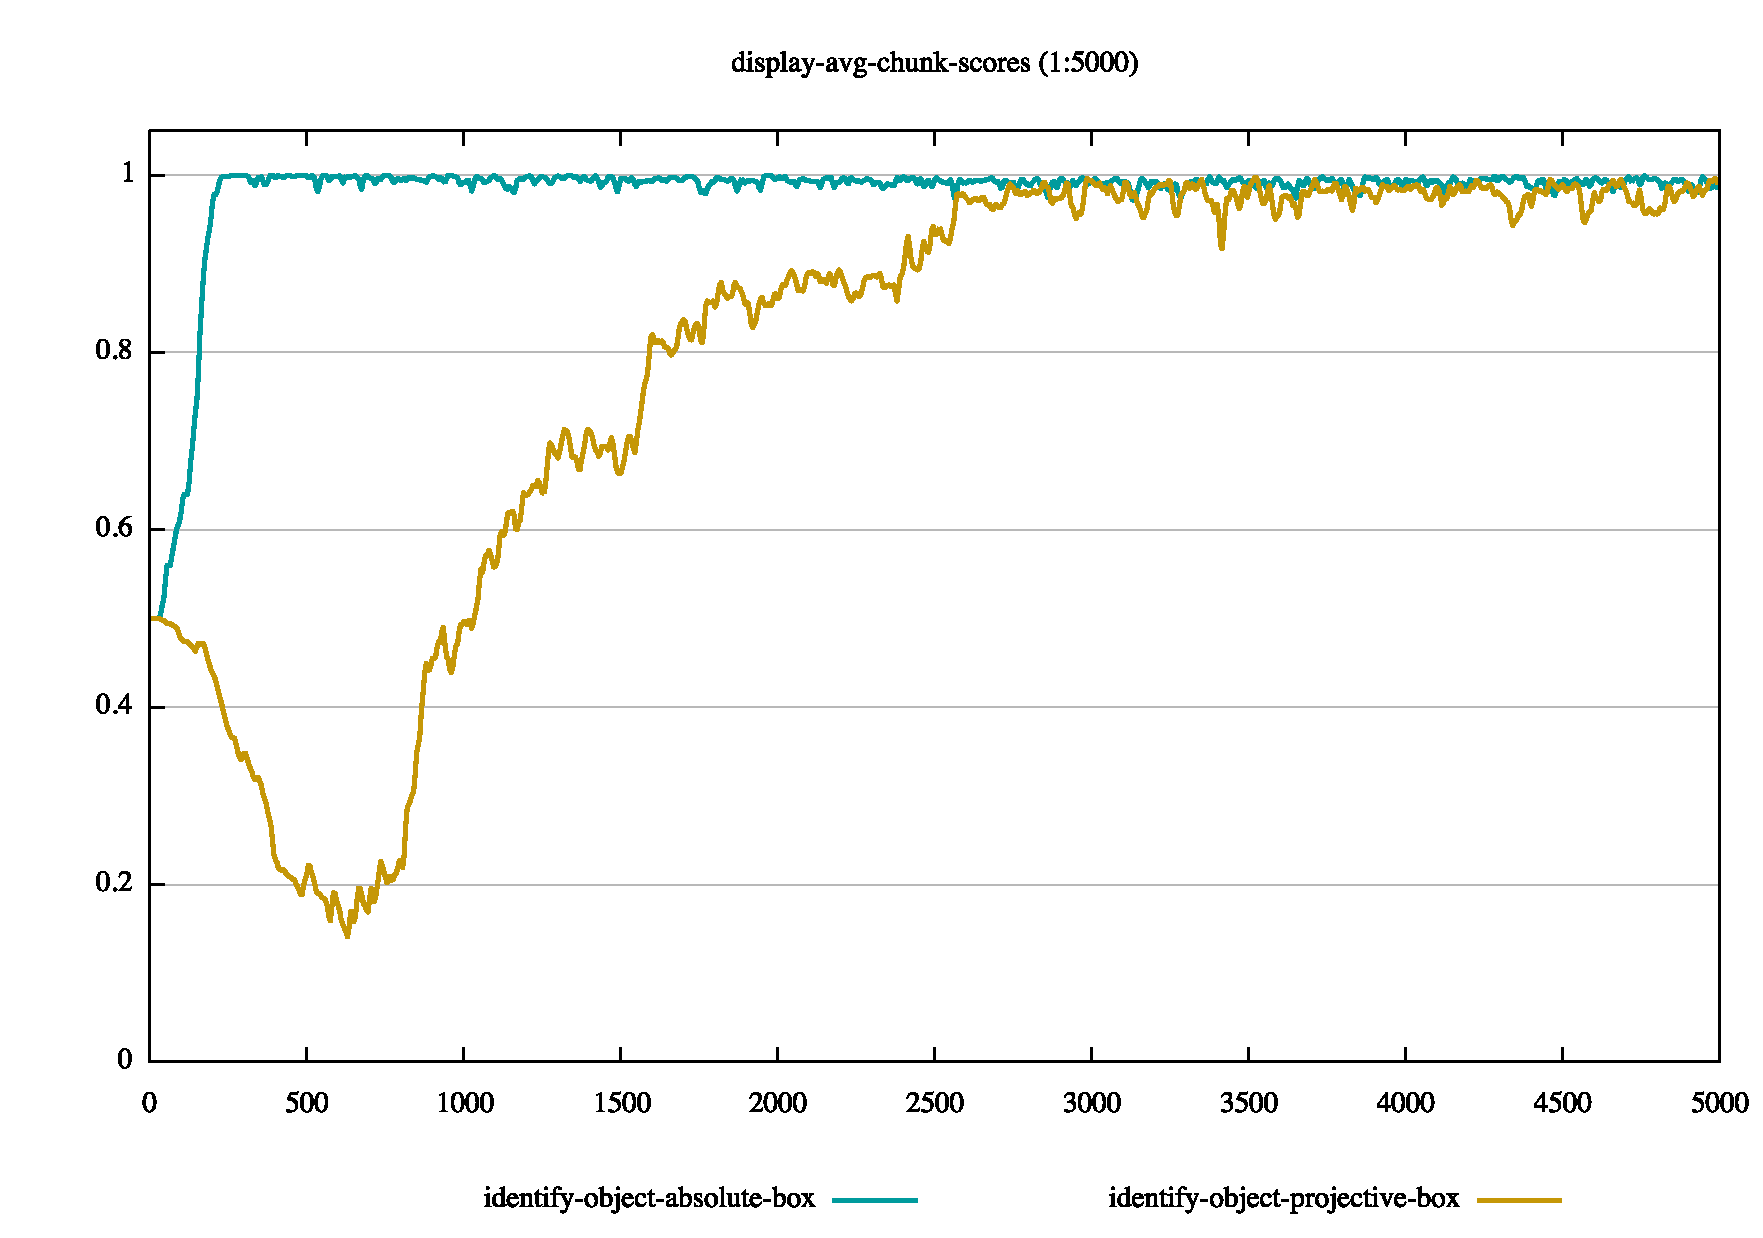
\includegraphics[width=0.7\columnwidth]{figs/chunk-alignment-frames-absolute-vs-intrinsic-05.pdf}
%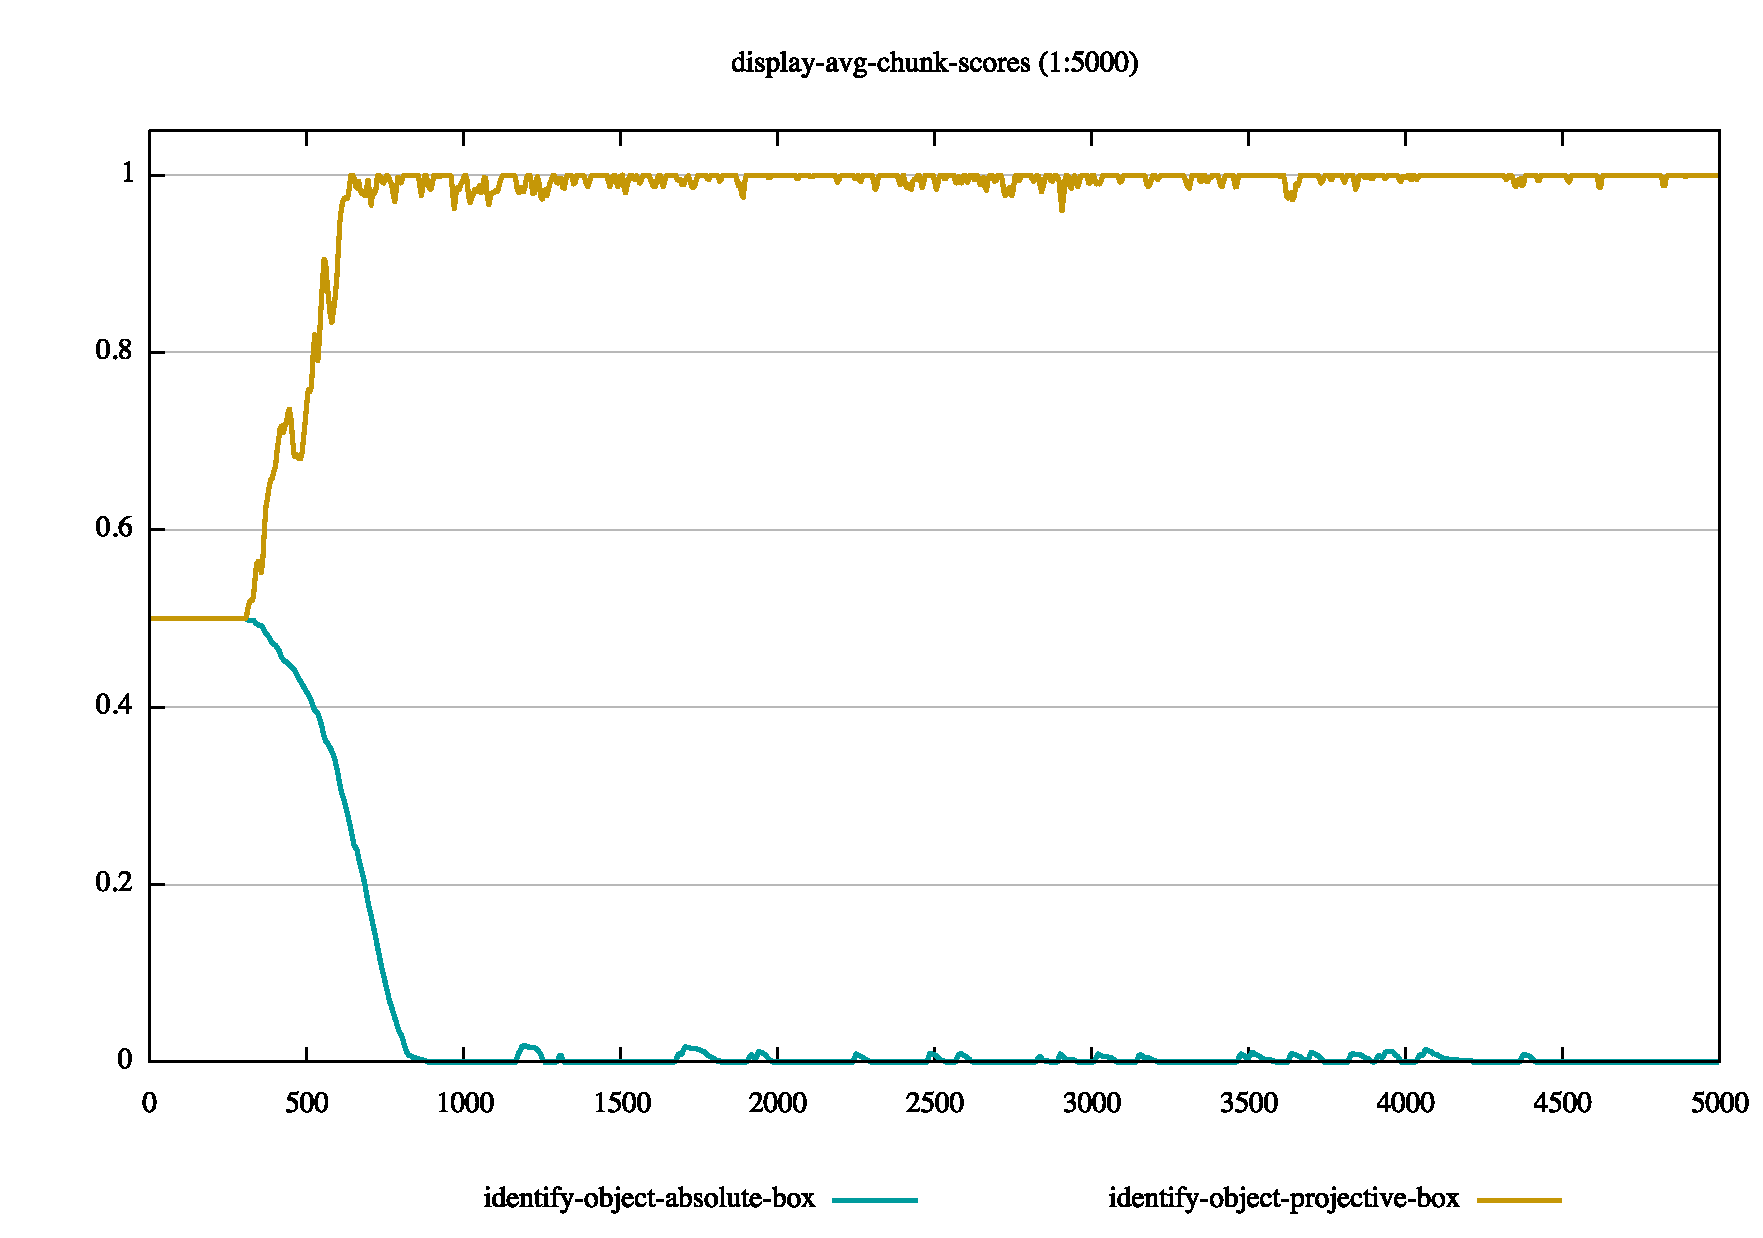
\includegraphics[width=0.7\columnwidth]{figs/chunk-alignment-frames-absolute-vs-intrinsic-10.pdf}
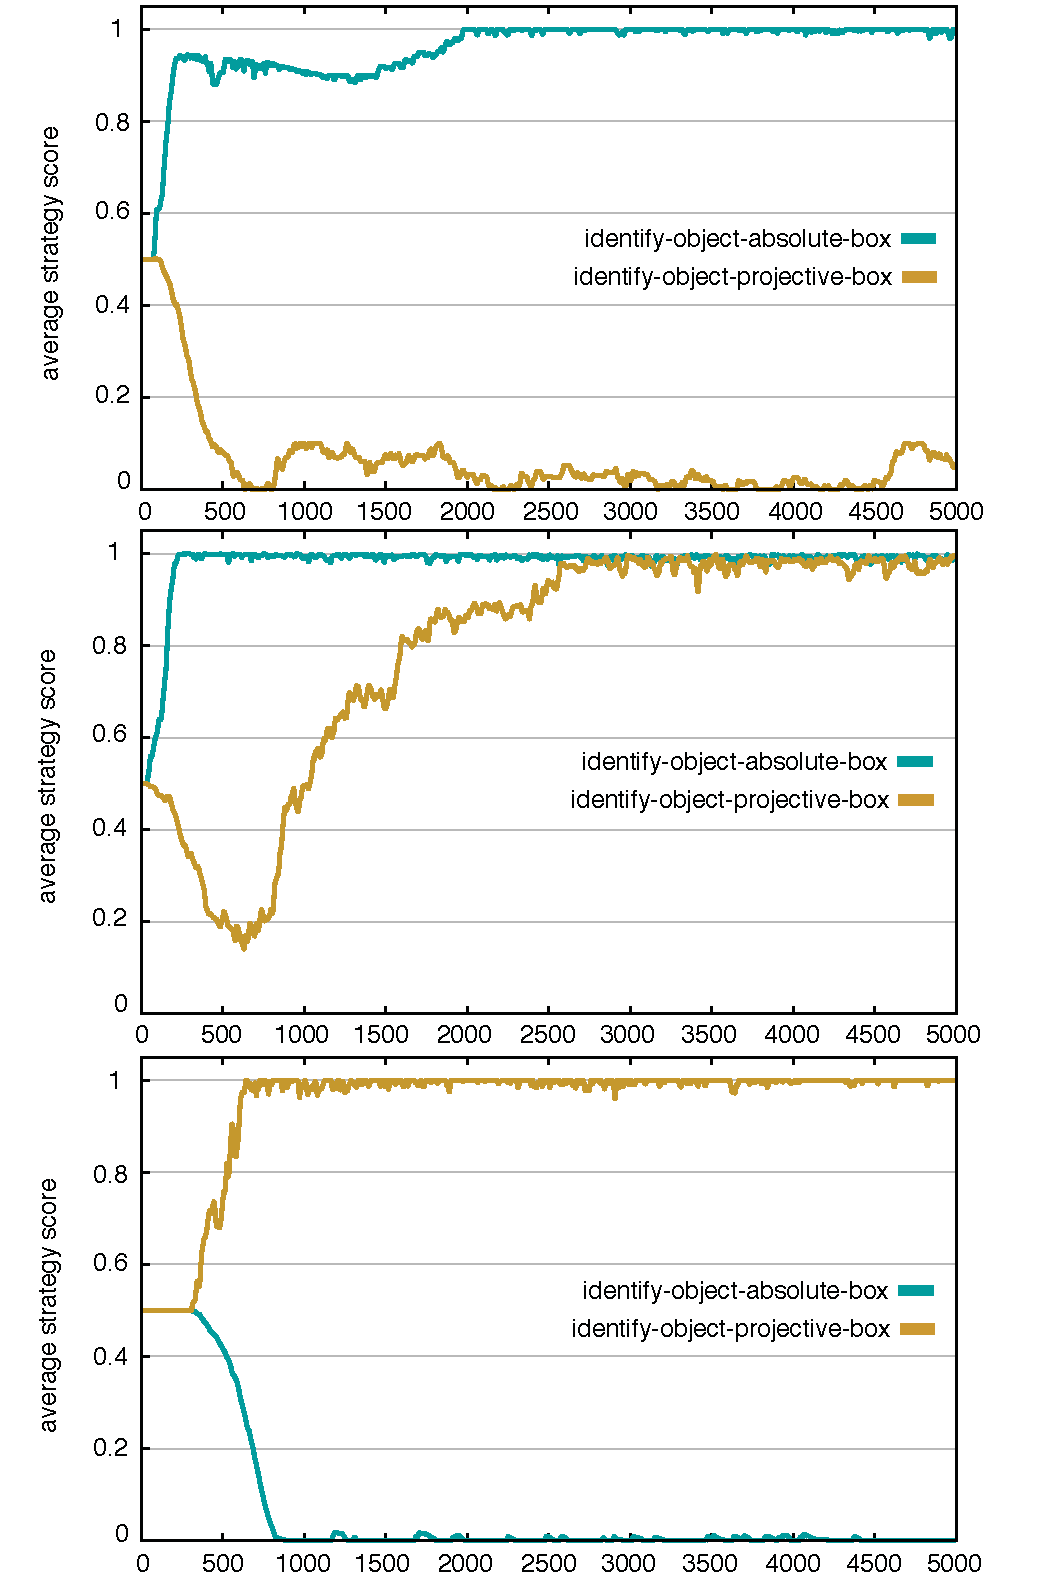
\includegraphics[width=0.8\columnwidth]{figs/chunk-alignment-frames-absolute-vs-intrinsic-together}
\end{center}
\caption[Dynamics of alignment\index{alignment} for different environmental conditions]{
Dynamics of alignment\index{alignment} for different environmental conditions. 
The graphs show the average score of the absolute and intrinsic strategy 
unfold over time. The top figure shows condition 0.0 (see Table 
\ref{t:conditions}, the middle figure shows 
condition 0.5, and the bottom figure shows condition 1.0.}
\label{f:chunk-alignment-frames-absolute-vs-intrinsic-detail}
\end{figure}

\begin{figure}
\begin{center}
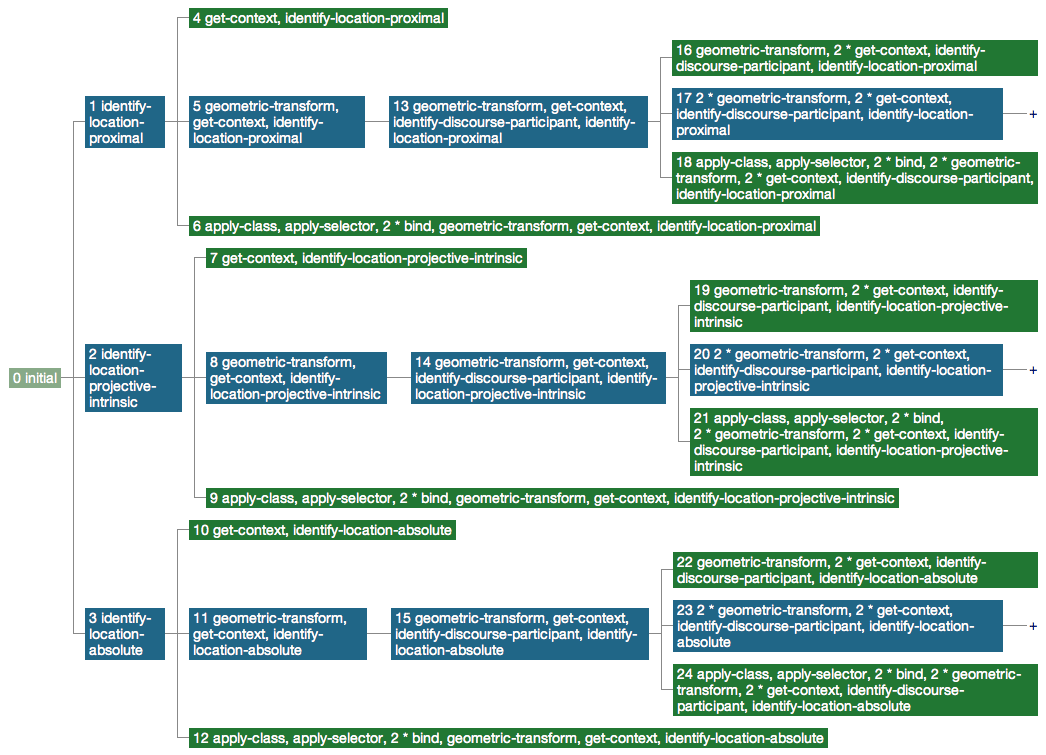
\includegraphics[width=1.0\columnwidth]{figs/conceptualization-strategy-invention-1.png}
\end{center}
\caption[Search for new conceptualization strategies]{
When agents are unable to conceptualize, they search for new 
conceptualization strategies by assembling cognitive operations 
into new chunks. Every node is a particular
semantic structure that is immediately tested using the current context and
the current topic. Here, different possible new strategies (green nodes) were found. 
Other possible strategies did not work on the current context (blue nodes).}
\label{f:strategy-invention-1}
\end{figure}

\begin{figure}
\begin{center}
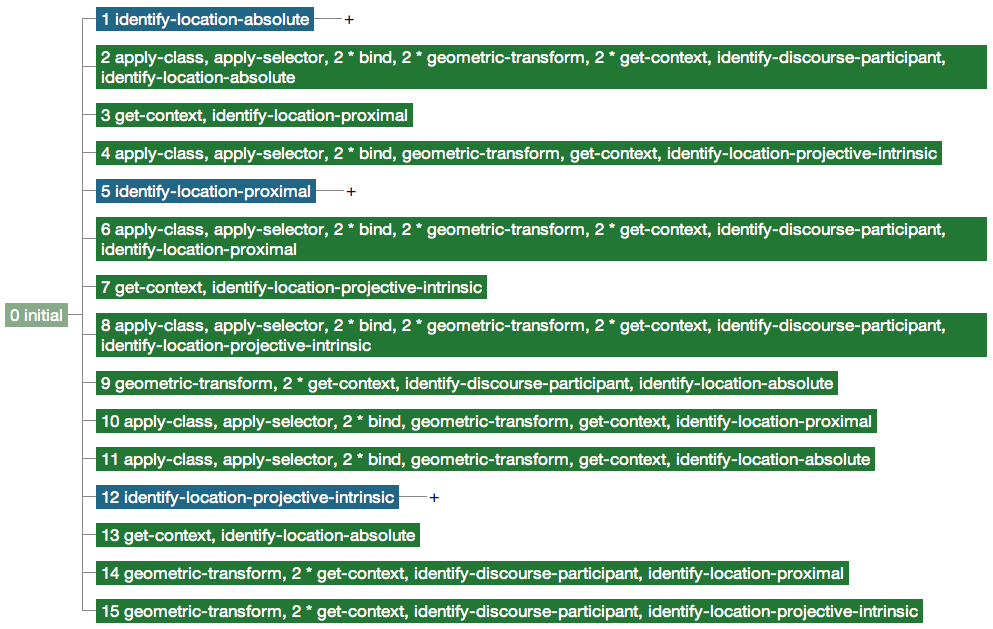
\includegraphics[width=1.0\columnwidth]{figs/conceptualization-strategy-invention-2.png}
\end{center}
\caption[Effect of new conceptualization strategies on the search process]{
The new strategies assembled by the agent (Figure \ref{f:strategy-invention-1})
are immediately stored in new chunks. This has the immediate effect of 
condensing the search process.
The new strategies are now in competition with each other, as well as with strategies 
already invented by the agent earlier. Which of these new strategies survives 
depends on the context and topic that agents are processing at the moment of invention.}
\label{f:strategy-invention-2}
\end{figure}

\section{Invention of Conceptualization Strategies}
The question of how conceptualization strategies can align in a population is important.
However, another important ingredient is, of course, how conceptualization strategies come
into existence in the first place. Invention is a necessary pre-requisite for the usage of
conceptualization strategies and their alignment\index{alignment} in a population. 
Invention of conceptualization strategies is based on the recruitment\index{recruitment} of basic cognitive operations
which are assembled into chunks. Once a chunk is invented, it immediately extends the conceptualization capabilities of agents. 
Invention of a particular conceptualization strategy is always 
based on a specific communicative situation, a specific context and a specific topic. 
The starting point for invention is a problem in communication. The agent is unable to conceptualize a 
meaning for some topic or the meaning that he was able to conceptualize is not discriminative enough. 
To solve the problem, the agent starts an elaborate search process (see Figures \ref{f:strategy-invention-1}
and \ref{f:strategy-invention-2})
which combines basic cognitive operations and the set of conceptualization 
strategies already established by the agent into new strategies. This process 
leads to new strategies, which are tested on the current context based on the
current communicative goal. The discriminative power of the new strategies decides if and
which strategy is stored for future use.

Strategy invention is deeply integrated into the processing of agents. 
Agents unable to conceptualize or unable to conceptualize with a sufficient discrimination
score diagnose a problem which is fixed by a repair that starts the search for new
conceptualization strategies.  The reason for this integration
with other invention mechanisms such as category invention is 
that agents when inventing new strategies also immediately have to invent new categories with
these strategies because the success of spatial strategies is tightly connected with the
spatial categories that are part of the strategy. This sort of dual invention 
is especially important in the beginning of experiments, when agents have neither developed 
strategies nor categories. But there is a second reason for deep integration of strategy invention. 
When an agent already has developed a strategy, he might also solve a particular
communicative problem by inventing new categories for these established strategies. 
Such decisions whether to use a new category
with an existing strategy or a new strategy with an existing category, or even to use
a newly invented strategy with a newly invented category are made based on the discriminative
power of each of these different possibilities. So, for instance, if an existing strategy has a low score,
the probability of inventing a new strategy increases, whereas if the current topic 
can be sufficiently discriminated using an existing strategy, no invention occurs.


Figure \ref{f:strategy-invention-dynamics} shows the process of invention and alignment of 
conceptualization strategies in a population of agents. In the experiment generating such results agents 
have a large repository of basic cognitive operations from which they can draw new building blocks 
whenever there are problems in communication. They can choose different landmarks: the robot or
the box and different category systems absolute and intrinsic projective as well as proximal.
The agents manage to agree on one particular strategy while at the same time developing a 
category system and a lexicon from scratch. The process, however, does not show the
same overall success as in the previously discussed experiments. The reason is that 
conceptual alignment is a difficult process which is complicated by the number 
of choices in strategies, population size (10 agents) and the variety 
of different contexts and discriminative situations which might all favor different strategies. 
In some contexts, proximal is the best strategy, some allow absolute and/or intrinsic categories 
to be invented. Nevertheless, agents do come to an agreement. Here, they agree on average on 
1 conceptualization strategy.

\begin{figure}
\begin{center}
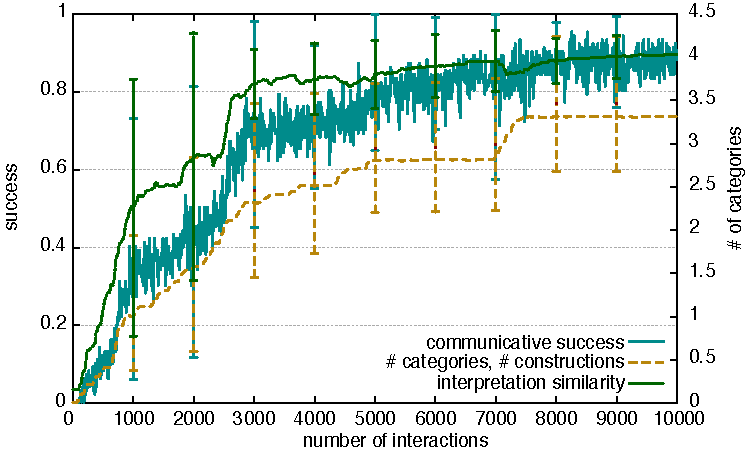
\includegraphics[width=0.9\columnwidth]{figs/chunk-alignment-category-invention-success}
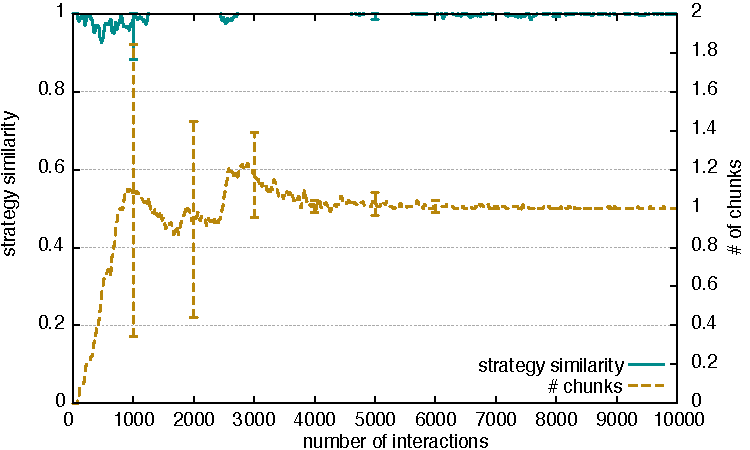
\includegraphics[width=0.9\columnwidth]{figs/chunk-alignment-category-invention-alignment}
\end{center}
\caption[Results for strategy invention, alignment and category development]{
Results for strategy invention, alignment and category development. A population
of 10 agents develops both conceptualization strategies as well as lexical systems for 
spatial strategies corresponding to these strategies.}
\label{f:strategy-invention-dynamics}
\end{figure}



\section{Discussion}
% is good can explain 1) emergence of single reference systems 2) self-organization of conceptualization
% strategies
Invention and alignment of conceptualization strategies are powerful processes that 
together allow agents to develop successful communication systems in the face of
varied environmental conditions. In turn, this allows agents to be more adaptive 
and ultimately more successful than the systems relying exclusively on categorization without 
taking into account reference objects, frames of reference and the different ways
of conceptualizing space. The study of conceptualization strategies is necessarily 
an important cornerstone in every theory of linguistic selection\index{selection} that has meaning as an important
part of the theory. The mechanisms proposed in this section are general enough that they
can, in principle, be applied to many different components of language, spatial language being only 
one of them. For the particular theory of linguistic selection\index{selection} pursued in this book, this 
section provides substantial evidence in the form of concrete computational experiments.
Language systems and in particular the conceptualization strategies underlying language systems, 
are the product of a cultural process based on the recruitment\index{recruitment} of cognitive operations 
and the environmental conditions the agents face.

This section shows that alignment of conceptualization strategies based on invention and selection\index{selection}
can be successful if the environment exhibits strong incentives for developing certain 
conceptualization strategies rather than others.
If this condition is met, discriminative power together with tracking the success of strategies,
which is the organizing principle used in this chapter,
can successfully orchestrate the self-organization\index{self-organization} of a complete lexical communication system
including the conceptualization strategy that gives rise to the communication system.
However, despite its success conceptual alignment has its limits, particularly in 
the approach presented here which relies exclusively on discrimination.
For instance, from a theoretical standpoint the relative conceptualization strategy
is the most dominant of the absolute, intrinsic and relative strategies. All these three strategies
have in common that they rely on angular relationships between objects and reference objects. 
The relative system in comparison to the other two angle based strategies however does not require additional 
intrinsic or absolute features, hence, in theory it is applicable in every 
spatial scene that features some landmark. This leads to a complete takeover of the 
relative system in experiments where relative, intrinsic and absolute systems compete
and where all scenes include a box landmark.
Table \ref{t:absolute-vs-intrinsic-vs-relative} summarizes
results in which certain spatial scenes have neither intrinsic nor absolute features.

\begin{table}
\caption[Results absolute, intrinsic and relative 
strategy competition]{
Results for absolute, intrinsic and relative 
conceptualization strategy competition
in different environmental conditions. This table shows 
communicative success and the
final scores of the relative, intrinsic and absolute 
strategy (all allocentric) after 10000 interactions 
(10 agents, 25 runs averaged).
Table \ref{t:experimental-conditions-absolute-vs-intrinsic-vs-relative} explains 
the different conditions.}
\begin{center}
\begin{tabular}{| p{1.5cm} | p{2.5cm} | p{1.5cm} | p{1.5cm}  | p{1.5cm} |}
\hline
condition & communicative success & score relative strategy 
& score intrinsic strategy & score absolute strategy\\ \hline\hline
0.25 & 100\% & 1.0 & 0.0 &  0.0\\ \hline
0.50 & 100\% & 1.0 & 0.0 &  0.0\\ \hline
0.75 & 100\% & 1.0 & 0.0 &  0.0\\ \hline
1.0 & 100\% & 1.0 & 0.0 &  0.0\\ \hline
\end{tabular}
\end{center}
\label{t:absolute-vs-intrinsic-vs-relative}
\end{table}

The strong advantage of relative frames of reference over other frames of reference 
hints at why relative frames of reference might have emerged, but it cannot explain why 
certain languages seem to prefer other types of frames of reference over the relative one.
Findings in natural language suggest, for example, that English speakers 
prefer the use of intrinsic frames of reference over relative frames of reference. 
The favored usage of intrinsic systems in English hints at the influence of  
important additional factors besides discrimination that govern the success of a particular strategy. One of such additional factors that was not studied in 
this section is cognitive complexity. For instance, 
relative systems are generally considered to be cognitively more 
demanding because they require tracking of perspective. It is relatively 
easy to add such constraints to the current
system, but running such experiments essentially requires one to 
put a number on how much one thinks the cognitive complexity of the 
relative systems is different from other strategies. To avoid such ad hoc 
quantities I did not pursue this idea. Nevertheless, based
on the experimental evidence described in this section, one can predict 
what will happen when factors additional to discriminative advantage 
are incorporated into the system. The mechanisms presented in 
this section function by packaging the successful 
conceptualization of a single context into strategies and tracking the success of
these strategies over many interactions, amplifying patterns in environmental conditions
and their effects over time and punishing rival strategies. Consequently, additional factors
favoring a particular strategy lead to faster and more stable alignment in the population.
So cognitive complexity, for instance, might be a factor that influences the alignment; 
in the best case, however, it leads to more robust alignment.


\begin{table}
\caption[Statistical distribution of features in the environment]{
Statistical distribution of features in the environment for
the different experimental conditions compared in Table \ref{t:absolute-vs-intrinsic-vs-relative}.}
\begin{center}
\begin{tabular}{ | l | p{1.5cm} | p{1.5cm} | p{1.5cm} | p{1.5cm} |}
\hline
condition & relative only & intrinsic + relative & absolute + relative & absolute + intrinsic + relative \\ \hline\hline
0.25 & 25\% & 30\% & 7.5\% & 37.5\%\\ \hline
0.50 & 50\% & 20\% & 5\% & 25\% \\ \hline
0.75 & 75\% & 10\% & 2.5\% & 12.5\% \\ \hline
1.0 & 100\% & 0\% & 0\% & 0\%\\ \hline
\end{tabular}
\end{center}
\label{t:experimental-conditions-absolute-vs-intrinsic-vs-relative}
\end{table}


Despite its success, conceptual alignment as presented in this section is a process
which requires the right conditions in order to flourish. Because agents not only develop 
strategies but also at the same time build category systems, the system is very powerful
and even in cases where there is almost no strategy alignment agents can
reach medium levels of communicative success\index{measures!communicative success}. The concurrent development of 
categories makes the system so powerful that in some cases alignment of strategies is prevented.
Consequently, agents can be rather successful even though the strategies they use are
not entirely the same. This brings us to another point: the role of exaptation. The underlying assumption
in all of the experiments in this section is that strategies co-evolve with the categories
and lexical systems from scratch. But often times new conceptualization strategies can re-use
existing material including categories as well as lexical and grammatical constructions 
and extend them to work within the new conceptual space that a strategy spans. This has been attested in 
spatial language which often is thought to originate in language for body parts (see 
for example \citealp{maclaury1989zapotec}\index{MacLaury, R. E.}). For the results in this section this means 
that the harsh condition that agents
start from virtually nothing can be relaxed. 
Applying this insight to exaptation one can predict that when systems become exapted 
and there are strong incentives for the population that direct invention of new strategies,
this has positive effects on the success and on alignment in conceptualization. 
A more detailed account of this phenomenon is, however, deferred to later sections.


The results presented in this section are interesting because they show that
agents can negotiate conceptualization strategies without marking them explicitly in
language. Indirect feedback via the spatial relations and the lexical system associated
with a particular spatial strategy are enough to allow the system to organize itself. 
However, an important factor of linguistic systems was deliberately avoided in the discussion so far:
the role of syntax. Many of the problems which cannot be solved by discrimination alone 
can be solved by agents when they are able to mark and express their strategies in more
complex ways than so far studied. The next sections picks up on this theme and gradually
introduce additional invention and learning mechanisms particular to the mapping from 
conceptualization strategies to syntactic structure.


% \bibliographystyle{diss}
% \bibliography{papers,space}
% \end{document}